\subsection{Technologien und Entscheidungen}

\subsubsection{Cordova Phonegap}

\subsubsection{HTML5}

\subsubsection{CSS}

\subsubsection{JS}

\subsubsection{Kartenmaterial}

Kartenmaterial im Browser bzw. der Hybrid-App ist ein essentieller Bestandteil von Location based Services. Durch eine Positionsbestimmung alleine erhält man nur Daten die für den Nutzer nicht anschaulich sind. Diese liegen normalerweise als geografische Koordinaten vor, die in geografischer Breite und geografischer Länge angegeben werden. Eine Beispielposition soll die Bedeutung von Kartenmaterial für den Nutzer von Location based Services verdeutlichen.

Als Beispiel hierfür wurde die Position der DHBW Mannheim in der Coblitzallee gewählt. Hierbei werden die geografischen Koordinaten, eine Adresse und ein Kartenausschnitt in einer Tabelle gegenübergestellt. Siehe hierzu Tabelle \ref{BedeutungVonKartenmaterial}.

\begin{table}[htbp]
\begin{center}
\begin{tabular}{|p{4.75cm}p{4.75cm}p{4.75cm}|} 
	\hline
		\rowcolor{black} \textcolor{white} { \textbf{Geographische Koordinaten} } & \textcolor{white}{\textbf{Adresse}} & \textcolor{white}{\textbf{Kartenausschnitt}}\\ 
		\rowcolor[gray]{.75}  49$^\circ$28'27.6\grqq N 8$^\circ$32'03.9\grqq E & Duale Hochschule Baden-Württemberg Mannheim \newline 
Coblitzallee 1-9 \newline 
68163 Mannheim \newline (Neuostheim) & Kartenausschnitt\newline 
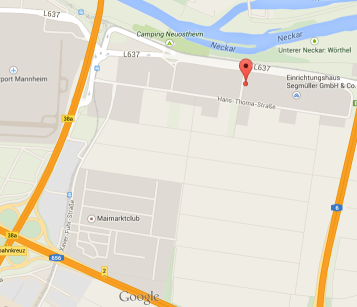
\includegraphics[width=0.3\textwidth]{ref/images/KartenmaterialKlein.png} \\ 
\hline
	\end{tabular}
\end{center}
\caption{Bedeutung von Kartenmaterial} \label{BedeutungVonKartenmaterial}
\end{table}

In der Tabelle sind verschiedenen Ortsdaten zur Verfügung gestellt, die alle Vor- und Nachteile aufweisen.

Die Geographischen Koordinaten geben die Position am genausten an, sind für fast keine Nutzer einer App von Bedeutung. 

Die Adresse ist im Alltag am geläufigsten und somit für Nutzer am verständlichsten. Allerdings ist die Angabe nicht so genau, wie die Geographischen Koordinaten. Denn die Angabe Hausnummer 1-9 gibt einen relativ großen Bereich an.

Die Vorteile eines Kartenausschnitts sind, dass die Detaillierung vom Nutzer angepasst werden kann. Des Weiteren werden viele grafische Informationen angezeigt, wie zum Beispiel der eigene Standort, an denen sich ein Nutzer Orientieren kann. Der Nachteil dieser Variante ist, dass die Kartenausschnitte die Zuhilfenahme von externen Quellen und einem erhöhten TODO: Programmieraufwand mit sich bringen.


TODO: Quelle finden
Auf Smartphones gehört Kartenmaterial und dessen Integration in Apps mittlerweile zum Standard, an welchen sich Nutzer gewöhnt haben. Aus diesem Grund sollte auch Kartenmaterial in die Location based Services App integriert werden, welche die Autoren bei dieser Studienarbeit entwickeln. 

Mögliche Quellen für das Kartenmaterial sind \glqq Google Maps\grqq, \glqq Bing Maps\grqq  und \glqq Open Street Maps\grqq.


\textbf{Anforderungen an das Kartenmaterial}

Die Anforderungen an interaktives Kartenmaterial bezüglich der in dieser Studienarbeit entwickeltem Projekt lassen sich in zwei Gruppen einteilen, die funktionalen und nichtfunktionalen Anforderungen.

Die \underline{nichtfunktionalen Anforderungen} sind:
\begin{enumerate}
\item Kostenlose Abfragen
\item Ohne Account nutzbar
\item Gute Dokumentation mit Codebeispielen
\item Zukunftssicherheit
\end{enumerate}

Die \underline{funktionalen Anforderungen} an das interaktive Kartenmaterial sind:
\begin{enumerate}
\item Eigenen Standort anzeigen
\item Markierungen auf der Karte setzen
\item Markierungen bündeln (optional)
\end{enumerate}

Bevor \glqq Google Maps\grqq, \glqq Bing Maps\grqq  und \glqq Open Street Maps\grqq bezüglich der Anforderungen untersucht werden, müssen diese genauer spezifiziert werden.

TODO: Hier Anforderungen erklären. Warum und wie die Umsetzung gewünscht ist.

Bsp.: Kostenlose Abfragen, da es sich nur um einen prototypische Implementierung handelt sollten bei der Entwicklung keine Kosten entstehen.
Bsp.: Ohne Account nutzbar, da studentisches Projekt mit mehr als einem Teammitglied
Bsp.: Gute Dokumentation mit Codebeispielen, da der Einstieg für die Entwickler leichter ist.
Bsp.: Zukunftssicherheit, da diese Arbeit nicht nur den aktuellen Stand der Technik abbilden soll, sondern auch einen Ausblick geben soll ist es wichtig, dass auch beim Kartenmaterial auf die Zukunftssicherheit geachtet wird.










